\section{Introduction}

Examples of deformable object manipulation range from domestic tasks like folding clothes to time and safety critical tasks such as robotic surgery. One of the challenges in planning for deformable object manipulation is the high number of degrees of freedom involved; even approximating the configuration of a piece of cloth in 3D with a 4 $\times$ 4 grid results in a 48 degree of freedom configuration space. In addition, the dynamics of the deformable object are difficult to model \citep{Essahbi2012}; even with high-fidelity modeling and simulation, planning for an individual task can take hours \citep{Bai2016}. Local controllers on the other hand are able to very efficiently generate motion, however, they are only able to successfully complete a task when the initial configuration is in the ``attraction basin'' of the goal \citep{Berenson2013,McConachie2018}.

\begin{figure*}[t]
    \centering
    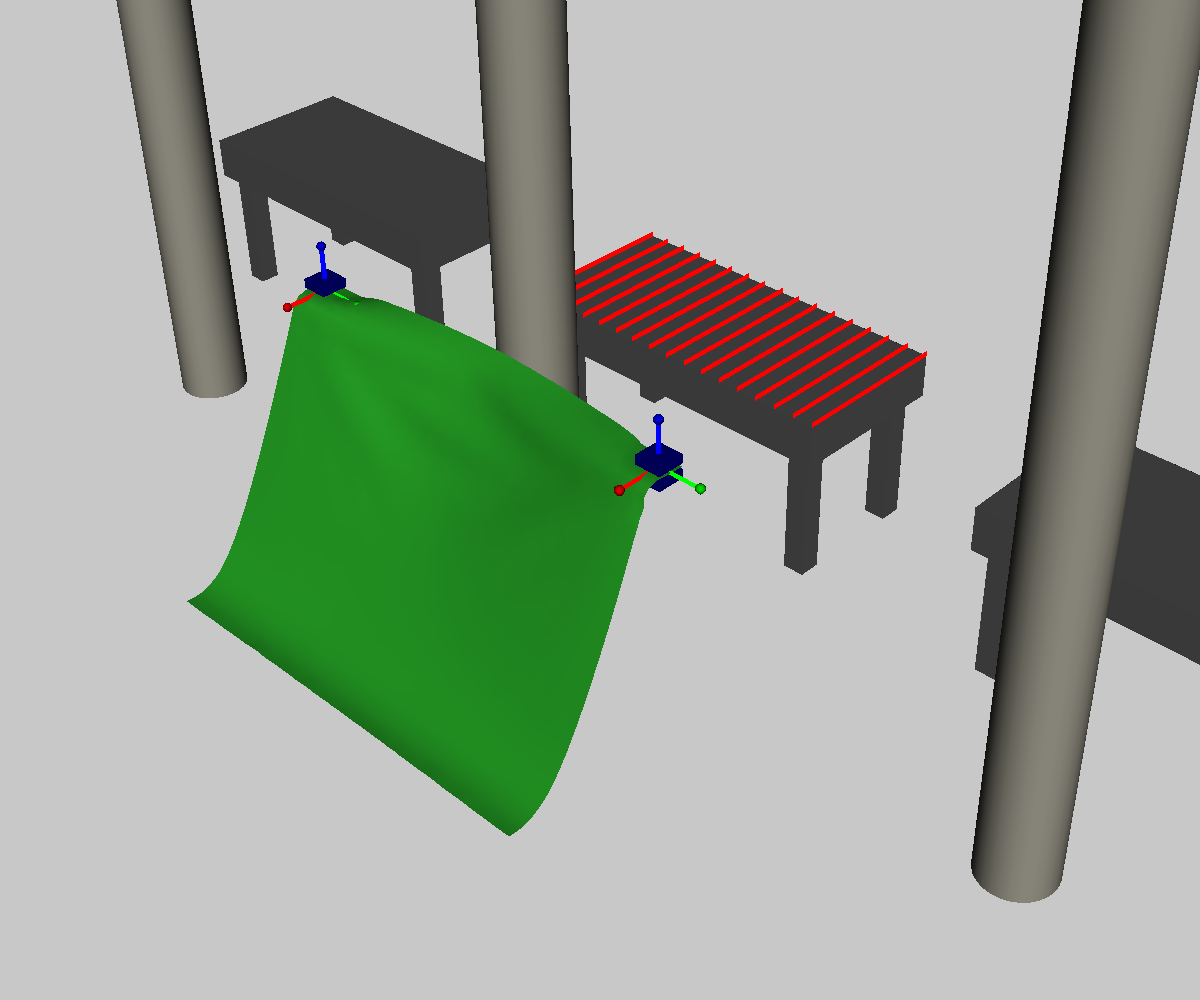
\includegraphics[trim={5cm 6cm 3cm 4cm},clip,width=0.24\textwidth,height=1.5in,keepaspectratio]{single_pole_starting_configuration}
    \hfill
    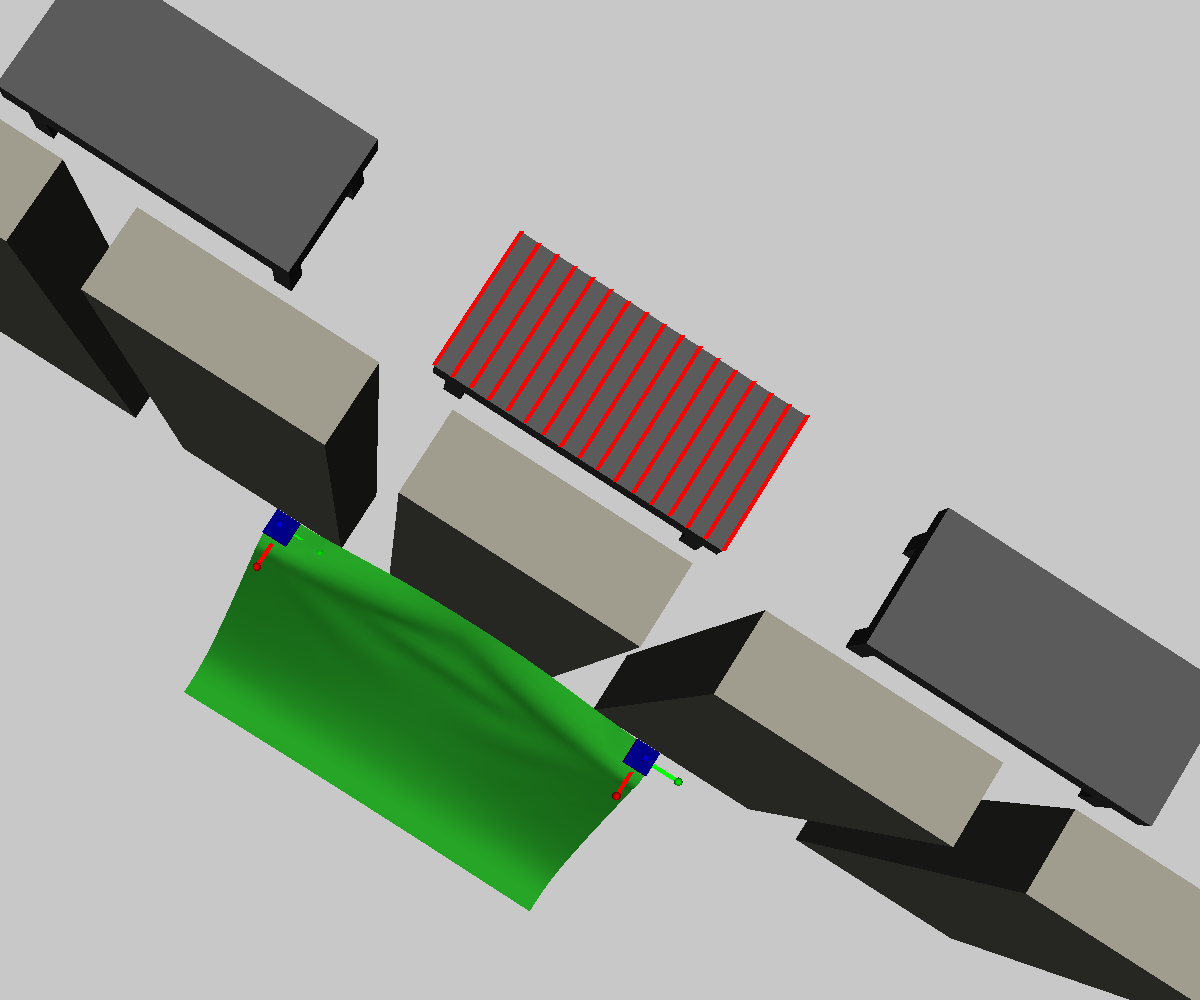
\includegraphics[trim={2cm 3cm 6cm 7cm},clip,width=0.24\textwidth,height=1.5in,keepaspectratio]{double_slit_starting_configuration}
    \hfill
    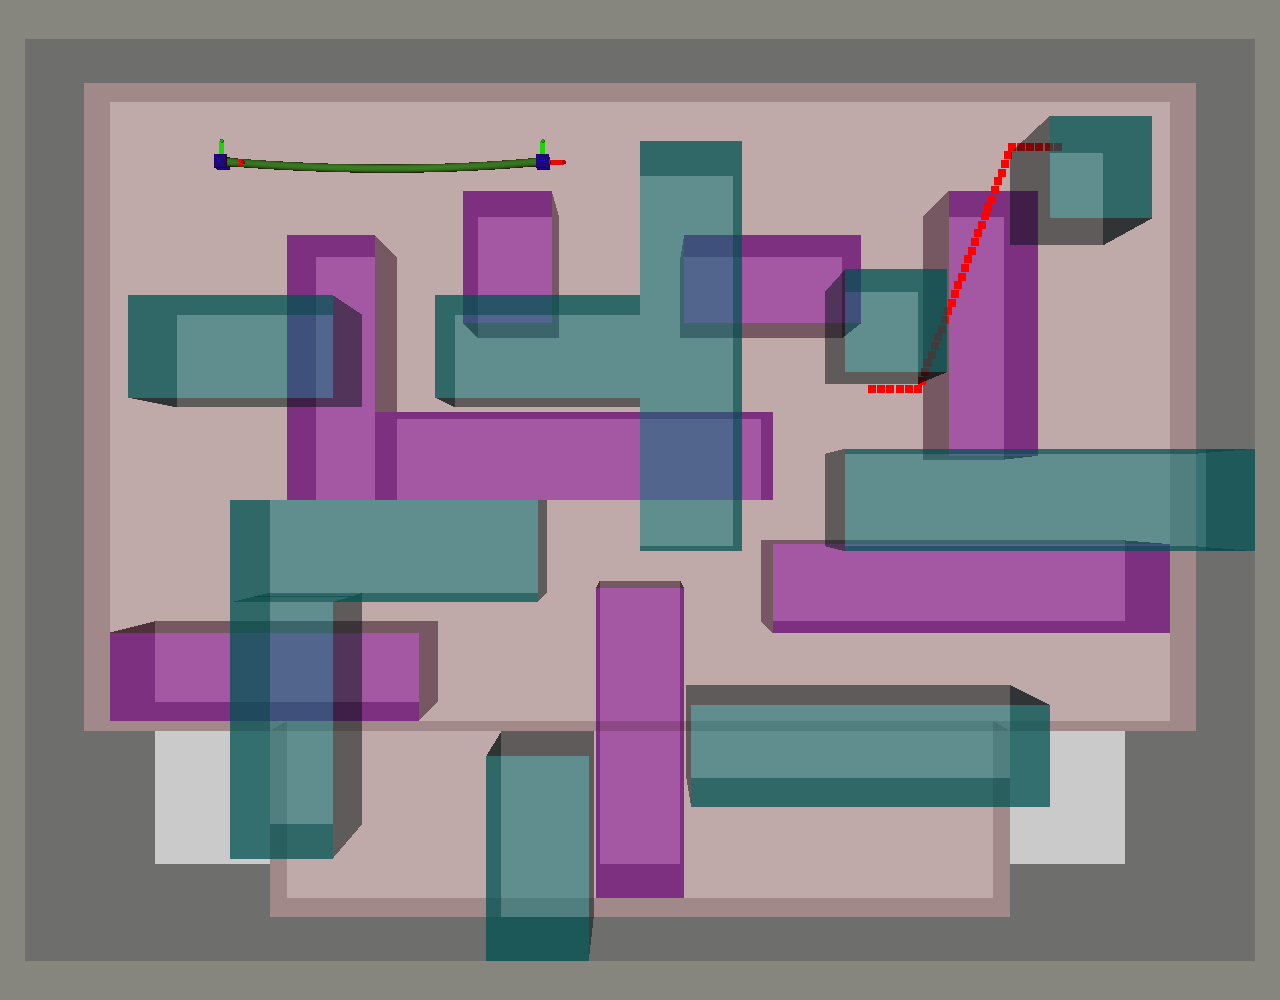
\includegraphics[trim={0cm 1cm 0cm 1cm},clip,width=0.24\textwidth,height=1.5in,keepaspectratio]{rope_maze_starting_configuration}
    \hfill
    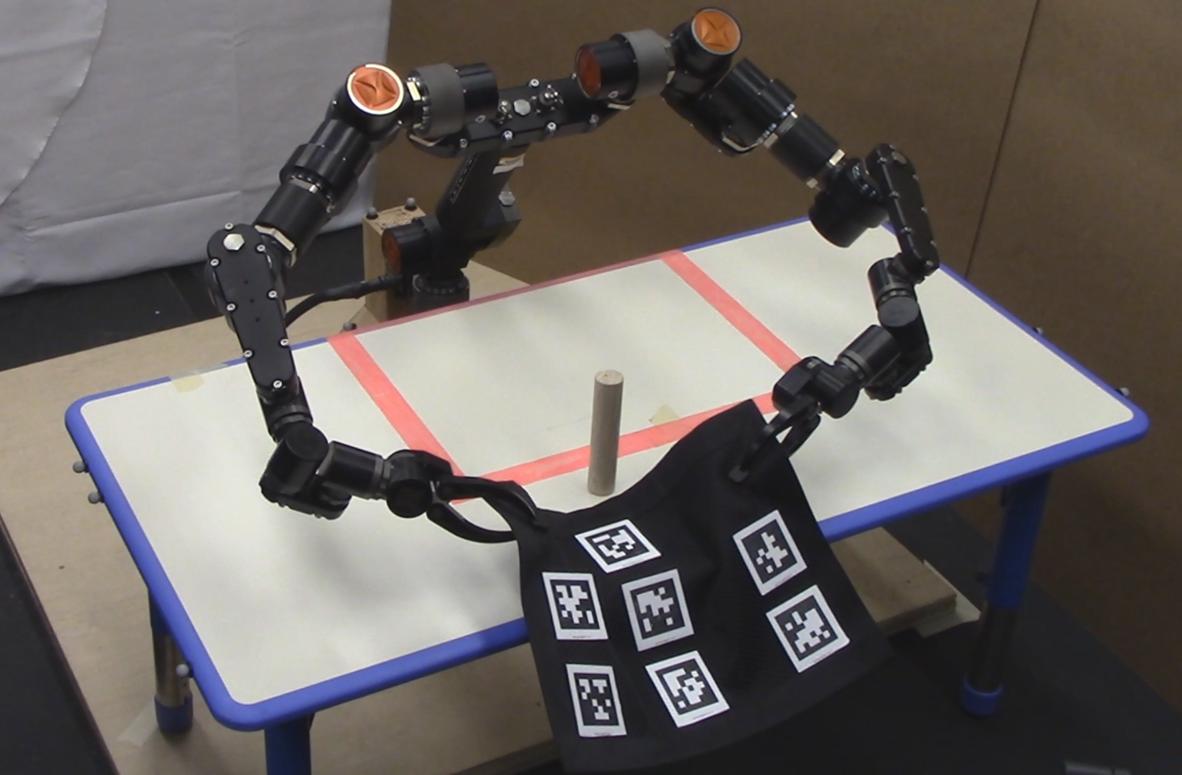
\includegraphics[trim={1.5cm 0cm 0.6cm 0cm},clip,width=0.24\textwidth,height=1.5in,keepaspectratio]{images/live_robot_starting_configuration}
    \caption{Four example manipulation tasks for our framework. In the first two tasks, the objective is to cover the surface of the table (indicated by the red lines) with the cloth (shown in green). In the first task, the grippers (shown in blue) can freely move however the cloth is obstructed by a pillar. In the second task, the grippers must pass through a narrow passage before the table can be covered. In the third task, the robot must navigate a rope (shown in green in the top left corner) through a three-dimensional maze before covering the red points in the top right corner. The maze consists of top and bottom layers (purple and green, respectively). The rope starts in the bottom layer and must move to the target on the top layer through an opening (bottom left or bottom right). For the fourth task, the physical robot must move the cloth from the far side of an obstacle to the region marked in pink near the base of the robot.}
    \label{fig:example_tasks}
\end{figure*}

The central question we address in this work is how can we combine the strengths of global planning with the strengths of local control while mitigating the weakness of each? We propose a framework for interleaving planning and control which uses global planning to generate gross motion of the deformable object, and a local controller to refine the configuration of the deformable object within the local neighborhood. By separating planning from control we are able to use different representations of the deformable object, each suited to efficient computation for their respective roles. In order to determine when to use each component, we introduce a novel deadlock prediction algorithm that is inspired by topologically-based motion planning methods \citep{Bhattacharya2012,Jaillet2008}. By answering the question ``Will the local controller get stuck?'' we can predict if the local controller will be unable to achieve the task from the current configuration. If we predict that the controller will get stuck we can then invoke the global planner, moving the deformable object into a new neighbourhood from which the local controller may be able to succeed. The key to our efficient prediction is forward-propagating only the stretching constraint, assuming the object will otherwise comply to contact.

We seek to solve problems for one-dimensional and two-dimensional deformable objects (i.e. rope and cloth) where we need to arrange the object in a particular way (e.g. covering a table with a tablecloth) but where there is also complex environment geometry preventing us from directly completing the task. While we cannot claim to solve all problems in this class (in particular in environments where the deformable object can be snagged), we can still solve practical problems where the path of the deformable object is obstructed by obstacles. In this work we restrict our focus to controllers of the form described in Sec.~\ref{sec:local_control}, and tasks suited to these controllers. Examples of these types of tasks are shown in Fig.~\ref{fig:example_tasks}. In our experiments we show that this iterative method of interleaving planning and control is able to successfully perform several interesting tasks where our planner or controller alone are unable to succeed.

Our contributions are: (1) A novel deadlock prediction algorithm to determine when a global planner is needed; (2) An efficient and probabistically-complete global planner for rope and cloth manipulation tasks; and (3) A framework to combine local control and global motion planning to leverage the strengths of each while mitigating their weaknesses. We present experiments in both a simulated environment and on a physical robot (Fig.~\ref{fig:example_tasks}). Our results suggest that our planner can efficiently find paths, taking under a second on average to generate a feasible path in three out of four simulated scenarios. The physical experiment shows that our framework is able to effectively perform tasks in the real world, where reachability and dual-arm constraints make the planning more difficult.

% \todo[inline]{You usually don't include smoothing when reporting planner time at this high level. You can say ``our planner finds a feasible path''. This is really what your planner is judged on. Smoothing is just icing on the cake.}

A preliminary version of this work was presented in \cite{McConachie2017}. This paper extends this work by adding an additional experiment on a physical robotic system as well as a proof of the probabilistic completeness of our planning method. We have also improved planning times with an improved goal bias method. We also include additional related work and an expanded discussion.